% ==================================================================================================================================
% Introduction

\minitoc  % Affiche la table des matières pour ce chapitre

Dans tout le début de ce chapitre, nous nous placerons dans un ensemble $E$ quelconque. 

% ==================================================================================================================================
% Espace Métrique

\section{Espace Métrique}

% -----------------------------------------
% Produit Scalaire

\subsection{Produit Scalaire}

Quand on parle de produit scalaire, on pense souvent à l'application dans le cas euclidien permettant de vérifier si 
deux vecteurs sont orthogonaux, en réalité, il existe une multitute de produits scalaires agissant sur tout autant d'espaces. 

\begin{definition}[Produit Scalaire]
    Soit $E$ un $\R$-espace vectoriel. Une application $\phi : E \times E \rightarrow \R$ de $E$ est un produit scalaire ssi c'est une forme :
    \begin{itemize}
        \item \textbf{Bilinéaire :} $ \forall x,y,z \in E, \forall \lambda,\mu \in \R$ on a :
            \begin{align}
                \phi(\lambda x + \mu y,z) = \lambda \phi(x,z) + \mu \phi(y,z) \\ 
                \phi(x,\lambda y + \mu z) = \lambda \phi(x,z) + \mu \phi(x,z)
            \end{align}
        \item \textbf{Symétrique :} $ \forall x,y \in E, \quad \phi(x,y) = \phi(y,x)$ 
        \item \textbf{Définie :} $ \forall x \in E, \quad \phi(x,x) = 0_\R \Longrightarrow x = 0_E $
        \item \textbf{Positive :} $ \forall x,y \in E, \quad \phi(x,y) \geq 0 $
    \end{itemize}
    On dit qu'un produit scalaire est une forme puisqu'elle est définie de E dans un corps telle que : 
        \[ \phi : E \longrightarrow \R \] 
    On note généralement un produit scalaire $ \langle .,. \rangle$ ou $(.|.)$. 
\end{definition}

\begin{remark}
    En pratique, pour montrer qu'une application est un produit scalaire, il suffit juste de montrer qu'elle est symétrique, 
    linéaire et définie positive. La bilinéarité découle de la symétrie et de la linéarité.  
\end{remark}

\begin{example}[Produits Sclaires]
    Regardons quelques exemples de produits scalaires...
    \begin{itemize}
        \item En génométrie euclidienne, on utilise un produit scalaire permettant de déterminer si deux vecteur sont 
        orthogonaux. Soient $A,B,C,D \in \R^2$, on définit alors :
            \[ \vec{AB}.\vec{CD} = AB \times CD \times \cos (\widehat{\vec{AB}\vec{CD}}) \]
        \item Dans l'espace des fonctions continues sur un intervalle $[a,b]$ on peut définir le produit scalaire suivant :
            \[ \forall f,g \in \mathcal{C}^0([a,b]), \quad \langle f,g \rangle = \int_{a}^{b} f(x)g(x) \; dx \] 
        \item Enfin, dans $\R^n$ on a le produit scalaire dit \textbf{euclidien} défini par : 
            \[ \forall x,y \in \R^n \text{ tels que : }
                \begin{cases}
                    x = (x_1, \dots, x_n) \\ 
                    y = (y_1, \dots, y_n)
                \end{cases}
                \text{ on a  : }
                \langle x,y \rangle = \sum_{i=1}^n (x_i y_i)^2 
            \] 
    \end{itemize}
\end{example}

\begin{prop}[Inégalité sur un produit scalaire]
    Soient $x,y \in E$, on a l'égalité suivante, valable pour tout produit scalaire :
        \[ \boxed{ \langle x,y \rangle ^2 \leq \langle x,x \rangle \times \langle y,y \rangle } \] 
\end{prop}

\begin{remark}
    Ce résultat découle de l'inégalité de Cauchy-Schwarz, vu plus tard. 
\end{remark}

% -----------------------------------------
% Norme

\subsection{Norme}

Une fois un produit scalaire défini sur un espace, on peut définir une application supplémentaire nous donnant plus d'informations 
sur un élément de l'espace. Nous allons donc définir une norme de deux façon, à partir d'un produit scalaire mais aussi 
de façon axiomatique. 

\begin{definition}[Norme]
    Soit $E$ un $\R$-espace vectoriel. Un application $\|.\| : E \rightarrow \R$ de $E$ est appelée \textbf{norme} ssi elle est : 
    \begin{itemize}
        \item \textbf{Définie : } $ \forall x \in E, \quad \|x \| = 0_\R \Longrightarrow x = 0_E $
        \item \textbf{Positive : } $ \forall x \in E, \quad \| x \| \geqslant 0 $
        \item \textbf{Positivement Homogène : } $ \forall x \in E, \forall \lambda \in \R, \quad \| \lambda x \| = |\lambda | \| x\| $  
        \item \textbf{Sous-additivité : } $ \forall x,y \in E, \quad \| x + y \| \leqslant \| x \| + \|y\| $
    \end{itemize}    
\end{definition}

\begin{remark}[Notation et vocabulaire]
    Tout comme le produit scalaire, une norme est une application vérifiant quelques propriétés. 
    Généralement, on note une norme $\|.\|$. Un espace muni d'une norme est appelé \textbf{espace normé}. 

    Dans un espace euclidien, une norme sert à "mesurer" la distance d'un point à l'origine. 
\end{remark}

\begin{example}
    Si on se place dans $\R$, le produit scalaire usuel sera la multiplication et la norme, la valeur absolue. 
\end{example}

\begin{proposition}[Norme à partir du produit scalaire]
    Dans un $\R$-espace vectoriel $E$, à partir d'un produit scalaire, on peut facilement définir une norme. 
    Soit $\langle .,. \rangle$ un produit scalaire sur $E$, alors l'application :
        \[
            \begin{cases}
                E \longrightarrow E \\
                x \longmapsto \sqrt{\langle x,x \rangle}
            \end{cases}
        \] 
    est une norme sur $E$. 
\end{proposition}

\begin{example}
    Dans $\R^n$, de même que le produit scalaire euclien, on peut définir la norme euclienne telle que :
    \[ 
        \forall x = (x_1, \dots, x_n) \in \R^n \quad \|x\| = \sqrt{ \sum_{i=1}^n (x_i)^2 }
    \] 
\end{example}

\begin{prop}[Inégalité de Cauchy-Schwarz]
    Soit $\langle .,. \rangle$ une produit scalaire sur $E$. On a alors l'inégalité suivante :
        \[ \boxed{ \forall x, y \in E, \quad | \langle x, y \rangle | \leqslant \| x\| \times \|y\| } \] 
    \emph{"La valeur absolue du produit scalaire est inférieure au produit des normes."}
\end{prop}

% -----------------------------------------
% Distance

\subsection{Distance et Espace Métrique}

Maintenant que nous pouvons "mesurer" des "longueurs" de vecteurs dans notre espace, on peut se demander si il est possible 
de "calculer" la distance entre deux éléments de $E$. Grâce à une telle application, on pourrait déterminer si deux éléments sont 
plus ou moins proches. Dès que l'on a une notion de distance, on peut ensuite l'intéresser à la notion de limite, etc... 

\begin{definition}[Distance]
    Soit $E$ un $\R$-espace vectoriel. 
    Une application $d(.,.) : E \times E \rightarrow \R$ est appelée \textbf{distance} ssi elle est :
    \begin{itemize}
        \item \textbf{Symétrique : } $ \forall x,y \in E, \quad d(x,y) = d(y,x) $
        \item \textbf{Définie : } $ \forall x,y \in E, \quad d(x,y) = 0_\R \Longrightarrow x = y $
        \item \textbf{Positive : } $ \forall x,y \in E, \quad d(x,y) \geqslant 0_\R $
        \item \textbf{Inégalité Triangulaire : } $ \forall x,yz \in E, \quad d(x,y) \leqslant d(x,z) + d(z,y)$ 
    \end{itemize}
\end{definition}

\begin{proposition}[Distance à partir d'une norme]
    Comme précédement, à partir d'une norme sur $E$, on peut facilement définir une distance entre deux vecteur. 
    Soit $\|.\|$ une norme sur $E$, l'application :
        \[ 
            \begin{cases}
                E \times E \longrightarrow \R \\ 
                (x,y) \longmapsto \| x - y \| 
            \end{cases}
        \] 
    Est une distance sur $E$. 
\end{proposition}

\begin{definition}[Espace Métrique]
    Un espace métrique est un couple $(E,d)$ où $E$ est un ensemble quelconque et $d$ une distance 
    sur cet ensemble.
\end{definition}

% ==================================================================================================================================
% Boules, Intérieur et Adhérence

\section{Boules, Intérieur et Adhérence}

Maintenant que nous savons "mesurer" des "longueurs" et déterminer à quels points deux éléments d'un espace sont 
"proches", nous pouvons introduire de nouveaux object à la base de tous les raisonnements que nous auront par la suite. 

Dans cette section, et pour la suite de ce cours, nous nous placerons dans des espaces métriques quelconques $(E,d)$ 
comme définis plus haut. 

\subsection{Boules}

Introduisons maintenant le concept de boule. 

\begin{definition}[Boule ouverte, fermée]
    Soit $a \in E, r \geqslant 0$ on appelle {boule ouverte} l'ensemble 
        \[ B(a,r) = \{ x \in E \; | \; \| x - a\| <  r\} \] 
    De même on définit la boule fermé comme l'ensemble :
    \[ \overline{B}(a,r) = \{ x \in E \; | \; \| x - a\| \leqslant r\} \] 
    On dit alors que $B(a,r)$ est la boule ouverte de rayon $r$ centrée en $a$ et 
    $\overline{B}(a,r)$ est la boule fermée de rayon $r$ centrée en $a$. 
\end{definition}

\begin{example}
    Pour tout $a \in \R$ on a :
        \[B(a,r) = \{ x \in E \; | \; \| x - a\| <  r\} = ]a - r ; a + r [ \]
        \[\overline{B}(a,r) = \{ x \in E \; | \; \| x - a\| \leqslant  r\} = [a - r ; a + r ] \]
\end{example}   

\begin{remark}
    En fonction de la norme (ou de la distance) choisie, une même boule peut avoir plusieurs formes. 

    \begin{center}
        \begin{tikzpicture}[scale=1.1]
            % Norme 2 (cercle)
            \begin{scope}[xshift=-3cm]
                \draw[->] (-1.5,0) -- (1.5,0) node[anchor=north west] {$x_1$};
                \draw[->] (0,-1.5) -- (0,1.5) node[anchor=south east] {$x_2$};
                \fill[pattern=north east lines, pattern color=gray!50] (0,0) circle (1);
                \draw[thick,black] (0,0) circle (1);
                \node at (0,-1.8) {Norme $\|.\|_2$};
            \end{scope}
        
            % Norme 1 (losange)
            \begin{scope}[xshift=0cm]
                \draw[->] (-1.5,0) -- (1.5,0) node[anchor=north west] {$x_1$};
                \draw[->] (0,-1.5) -- (0,1.5) node[anchor=south east] {$x_2$};
                \fill[pattern=horizontal lines, pattern color=gray!50] (0,1) -- (1,0) -- (0,-1) -- (-1,0) -- cycle;
                \draw[thick,black] (0,1) -- (1,0) -- (0,-1) -- (-1,0) -- cycle;
                \node at (0,-1.8) {Norme $\|.\|_1$};
            \end{scope}
        
            % Norme infinie (carré)
            \begin{scope}[xshift=3cm]
                \draw[->] (-1.5,0) -- (1.5,0) node[anchor=north west] {$x_1$};
                \draw[->] (0,-1.5) -- (0,1.5) node[anchor=south east] {$x_2$};
                \fill[pattern=vertical lines, pattern color=gray!50] (-1,-1) rectangle (1,1);
                \draw[thick,black] (-1,-1) rectangle (1,1);
                \node at (0,-1.8) {Norme $\|.\|_\infty$};
            \end{scope}
        \end{tikzpicture}    
    \end{center}
\end{remark}

\subsection{Intérieur et Adhérence}


\begin{definition}[Intérieur]
    Soit $A \subset E$, soit $a \in E$, on dit que $a$ est intérieur à $A$ ssi 
        \[ \boxed { \exists \varepsilon > 0, \quad B(a,\varepsilon) \subset A } \] 
    Autrement dit, $a$ est intérieur à $A$ ssi on peut construire une boule autour de $a$ qui 
    soit entièrement contenue dans $A$. 

    On dit alors que $A$ est voisinnage de $a$. L'ensemble des points intérieurs d'une partie est appelé 
    l'intérieur de cette partie. On le note $int(.)$. 
\end{definition}

\begin{definition}[Adhérence]
    Soit $A \subset E$, soit $a \in E$, on dit que $a$ est adhérent à $A$ ssi 
        \[ \boxed { \forall \varepsilon > 0, \quad B(a,\varepsilon) \cap A \not = \emptyset } \] 
    Autrement dit, $a$ est adhérent à $A$ ssi pour toute boule autour de $a$, cette boule est intersectée avec $A$
    (i.e on ne peut pas construire de boule autour de $a$ qui ne "déborde" pas sur $A$).

    On dit alors que $a$ est dans l'adhérence de $A$. L'adhérence d'une partie est l'ensemble de ses points adhérents. 
    On le note $adh(.)$.
\end{definition}

\begin{remark}[Illustration]
    Soit $A \subseteq E$ et $x,y \in E$ tels que $x$ soit intérieur à $A$ et $y$ soit adhérent à $A$. 
    On pourrait représenter cela par le dessin ci-dessous :

    \begin{center}
        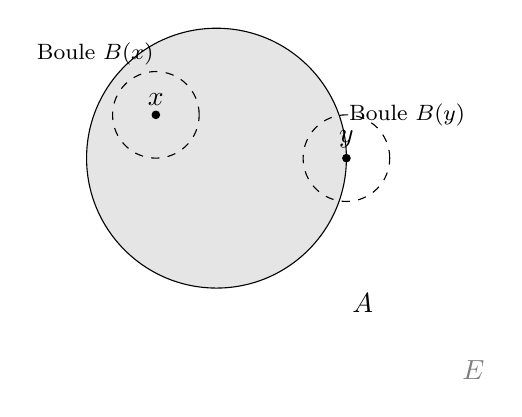
\begin{tikzpicture}[scale=1.1]
            % Partie A
            \draw[fill=gray!20,draw=black] (0,0) circle (1.5) node[below right=1.6cm, black] {$A$};
        
            % Point intérieur à A
            \fill[black] (-0.7,0.5) circle (0.05) node[above] {$x$};
            \draw[black, dashed] (-0.7,0.5) circle (0.5);
            \node[black] at (-1.4,1.2) {\footnotesize Boule ${B}(x)$};
        
            % Point adhérent à A mais pas intérieur
            \fill[black] (1.5,0) circle (0.05) node[above] {$y$};
            \draw[black, dashed] (1.5,0) circle (0.5);
            \node[black] at (2.2,0.5) {\footnotesize Boule ${B}(y)$};
        
            % Indication du fond (l'ensemble $E$)
            \node[below right=3cm, gray] at (0,0.5) {$E$};
        
            % Légendes
            % \draw[fill=blue!20, draw=blue, opacity=0.3] (-2.8,-2) rectangle (-1.8,-1.5);
            % \node[anchor=west] at (-1.7,-1.75) {\footnotesize Partie $A$};
            % \fill[red] (-2.8,-2.5) circle (0.1);
            % \node[anchor=west] at (-1.7,-2.5) {\footnotesize Intérieur ($x$)};
            % \fill[green] (-2.8,-3) circle (0.1);
            % \node[anchor=west] at (-1.7,-3) {\footnotesize Adhérent ($y$)};
        \end{tikzpicture}
    \end{center}

    L'intérieur d'une partie peut se voir comme l'ensemble des points "profonds" de cette partie. 
    Au contraire l'adhérence peut se voir comme tous les points qui sont dedans et "très proches". 
\end{remark}

\begin{definition}[Frontière]
    Soit $A \subseteq E$, on définit la frontière comme l'ensemble :
        \[ \partial A = adh(A) / int(A) \] 
\end{definition}

\begin{example}
    Soit $A$ le disque ouvert de rayon 1 dans $\R^2$. Déterminons son intérieur, son adhérence et sa frontière. 
        \[ A := \{ (x,y) \in \R^2 \; | \; x^2 + y^2 < 1 \} \] 
    On a : 
    \begin{itemize}
        \item $adh(A) = \{ (x,y) \in \R^2 \; | \; x^2 + y^2 \leqslant 1 \} $
        \item $int(A) = \{ (x,y) \in \R^2 \; | \; x^2 + y^2 \leqslant 1 \} = A $
        \item $\partial A = \{ (x,y) \in \R^2 \; | \; x^2 + y^2 = 1 \} $
    \end{itemize}
\end{example}

\begin{proposition}
    Soit $A \subset (E,d)$ $int(A)$ est le plus ouvert contenu dans $A$ et $adh(A)$ est le plus petit 
    fermé de $E$ contenant $A$. 
\end{proposition}


\subsection{Propriétés}

\begin{proposition}
    L'intérieur d'une boule ouverte est la boule fermée correspondante. 
\end{proposition}

\begin{prop}[Inclusions et complémentaire]
    Soit $E$ un espace métrique et $A,B \subseteq E$. 
    \begin{itemize}
        \item Si $A \subset B$ on a alors :
            \[ int(A) \subset int(B) \quad adh(A) \subset adh(B) \] 
        \item $int(A) = \overline{(adh(\overline{A}))} $ et $ adh(A) = \overline{(int(\overline{A}))}$ 
        \item 
        \begin{itemize}
            \item $ int(A \cup B) \supset int(A) \cup int(B) $
            \item $ int(A \cap B) = int(A) \cap int(B) $
            \item $ adh(A \cup B) = adh(A) \cup adh(B) $
            \item $ adh(A \cap B) \subset adh(A) \cap adh(B) $
        \end{itemize}
    \end{itemize}
\end{prop}

\begin{proposition}[Adhérence et sup dans le cas réel]
    Soit $A \subset \R$, non vide et majorée alors, $\sup (A) \in adh(A)$. 
\end{proposition}

% ==================================================================================================================================
% Suites et Limites

\section{Suites et Limites}

\subsection{Généralités}

Définissons clairement la notion de suite numérique. 

\begin{definition}[Suite Numérique]
    Soit $I \subseteq \N$ une \textbf{partie infinie}. 
    On appelle suite à valeurs dans $(E,d)$, un espace métrique, d'ensemble d'indices $I$, 
    toute application : 
        \[ (u_n)_{n \in I} : n \longrightarrow u_n \in E \] 
    On dit alors que $u_n$ est le \emph{terme d'indice} $n \in I$. 
    On note $E^I$ l'ensemble des suites à valeurs dans $E$ d'ensemble d'indices $I$.  
\end{definition}

\begin{example}
    On a par exemple : 
    \begin{itemize}
        \item La suite $(u_n)_{n \in \N}$ définie $ \forall n \in \N$ par $u_n = \sqrt{4n + 1}$. 
        \item La suite $(u_n)_{n \in \N^*}$ définie par $u_n = \ln(n + 2n^2)$. 
    \end{itemize}
\end{example}

\begin{remark}
    Par abus de notation on notera souvent $(u_n)$ pour désigner une suite. L'ensemble d'indices et 
    les valeurs que prennent la suite dépendront du contexte. 

    Attention, il faut toutefois bien différentier la suite $(u_n)$ de son terme général noté $u_n$ 
    qui correspond à une valeur de la suite pour un certain $n \in I$. 
    En effet, le premier élément $(u_n)$ appartient à $E^I$ alors que le second appartient à $E$. 
\end{remark}

\begin{proposition}
    Soit $(u_n)_{n \in I}$ à valeur dans $E$. Si $E = \R$ on dira que la suite $(u_n)$ est 
    \emph{à valeurs réelles}. 
\end{proposition}

\subsection{Propriétés}

Nous allons ici nous concentrer sur les suites à \emph{valeurs réelles}. 
En effet, la relation d'ordre $\leqslant$ dans $\R$ nous permettra de comparer différentes valeurs 
d'une suite et ainsi de définir le concept de monotonie. 

\begin{definition}[Monotonie]
    Soit $(u_n)_{n \in I}$ une suite à valeurs réelles d'ensemble d'indices $I \subseteq \N$. 
    \begin{enumerate}
        \item On dit que $(u_n)$ est \emph{croissante} (resp. strictement croissante) si 
            \[ \forall n \in I, \quad u_{n+1} \geqslant u_n \quad (\text{resp. } u_{n+1} > u_n) \] 
        \item On dit que $(u_n)$ est \emph{décroissante} (resp. strictement décroissante) si 
            \[ \forall n \in I, \quad u_{n+1} \leqslant u_n \quad (\text{resp. } u_{n+1} < u_n) \] 
        \item On dit que $(u_n)$ est \emph{constante} si : 
            \[ \exists C \in \R, \quad \forall n \in I, \quad u_n = C \] 
        \item On dit que $(u_n)$ est \emph{stationnaire} si : 
            \[ \exists C \in \R, \quad \exists N \in \N, \quad \forall n \geqslant N, u_n = C \] 
        \item On dit que $(u_n)$ est \emph{périodique} si : 
            \[ \exists p \in \N^*, \quad \forall n \in \N, \quad u_n = u_{n+p} \] 
    \end{enumerate}
\end{definition}

\begin{remark}
    Dans le cadre de la définition suite : 
    \begin{enumerate}
        \item Étudier la monotonie d'une suite revient donc à dire si elle est croissante ou décroissante. 
        \item On parlera de suite \emph{monotone} lorsqu'elle sera uniquement croissante OU décroissante. 
            Toutes les suites ne sont donc pas monotones. 
        \item Une suite stationnaire est une suite constante à partir d'un certain rang (noté $N$ dans la définition). 
    \end{enumerate}
\end{remark}

\begin{definition}[Suite Majorée, Minorée, Bornée]
    Soit $(u_n)_{n \in I}$ une suite à valeurs réelles d'ensemble d'indices $I \subseteq \N$. 
    \begin{enumerate}
        \item On dit que $(u_n)$ est \emph{majorée} si : 
            \[ \exists M \in \R, \quad \forall n \in I, \quad u_n \leqslant M \] 
            On dira que $M$ est le majorant de $(u_n)$. 
        \item On dit que $(u_n)$ est \emph{minorée} si : 
            \[ \exists m \in \R, \quad \forall n \in I, \quad u_n \geqslant m \] 
            On dira que $M$ est le minorant de $(u_n)$. 
        \item On dit que $(u_n)$ est \emph{bornée} si : 
            \[ \exists B \in \R, \quad \forall n \in I, \quad | u_n | \leqslant B \]
    \end{enumerate}
\end{definition}

\begin{proposition}
    Soit $(u_n)_{n \in \N}$ une suite à valeurs réelles. 
    Alors $(u_n)$ est bornée ssi elle est majorée ET minorée. 
\end{proposition}

\subsection{Convergence et Limites de Suites Numériques}

\begin{definition}[Limite et Suite Convergente]
    Soit $(u_n)$ une suite numérique. 
    \begin{enumerate}
        \item On dit que $(u_n)$ \emph{converge} ou \emph{tend} vers $l \in \R$ si 
            \[ \forall \varepsilon > 0, \quad \exists N \in \N, \quad \forall n \in \N, \quad n \geqslant N \Longrightarrow |u_n - l| < \varepsilon \]  
            On notera alors $ \underset{n \to \infty}{\lim} u_n = l$ ou $ u_n \underset{n \to \infty}{\longrightarrow} l$. 
        \item On dit que $(u_n)$ est \emph{convergente} si : 
            \[ \exists l \in \R, \quad \forall \varepsilon > 0, \quad \exists N \in \N, \quad \forall n \in \N, \quad n \geqslant N \Longrightarrow |u_n - l| < \varepsilon \] 
            On utilisera la même notation que précédement. 
        \item On dit que $(u_n)$ est \emph{divergente} si elle n'est pas convergente : 
            \[ \forall l \in \R, \quad \exists \varepsilon > 0, \quad \forall N \in \N, \quad \exists n \in \N, \quad n \geqslant N \text{ et } |u_n - l| \geqslant \varepsilon \] 
    \end{enumerate}
    On peut facilement étendre cette définition aux limites infinies.
\end{definition}

\begin{prop}[Unicité de la limite]
    Soit $(u_n)$ une suite numérique. 
    Si $(u_n)$ converge vers une limite $l \in \R$ et qu'elle converge aussi vers une autre limite $l' \in \R$ alors 
    $l = l'$. C'est ce que l'on appelle l'unicité de la limite. 
\end{prop}

\begin{prop}[Limites et Majoration/Minoration]
    Soit $(u_n)$ une suite à valeurs réelles. 
    \begin{itemize}
        \item Si $(u_n)$ converge, alors $(u_n)$ est bornée. 
        \item Si $u_n \underset{n \to \infty}{\longrightarrow} + \infty$ (resp. $- \infty$) alors $(u_n)$ n'est pas majorée (resp. minorée). 
    \end{itemize}
\end{prop}

\begin{prop}[Convergence et suites partielles]
    Toute suite partielle d'une suite convergente est convergente et converge vers la même limite. 
\end{prop}

\begin{definition}[Suite de Cauchy]
    Soit $(E,d)$ un espace métrique et $(u_n)_{n \in \N}$ une suite à valeurs dans $E$. 
    On dit que $(u_n)$ est \emph{de Cauchy} ou \emph{une suite de Cauchy} lorsque ses termes 
    se rapprochent uniformément les uns des autres lorsque $n$ tend vers $ + \infty$. 
        \[ i.e \quad \lim_{p,q \to \infty} d(u_p, u_q) = 0 \] 
        \[ \iff \forall \varepsilon > 0, \; \exists N \in \N, \; \forall q \geqslant N, \; \forall q \geqslant N, \quad d(u_p,u_q) < \varepsilon \]  
\end{definition}

\begin{remark}
    Attention : il ne suffit pas que la différence des termes consécutifs de la suite tendent vers zéro. 
    Les suites de Cauchy ne sont pas à confondre avec les suites convergentes. En effet, une suite convergente 
    est de Cauchy mais la réciproque est fausse. 
\end{remark}

\begin{example}
    Soit $(u_n)$ une suite décroissante de rationnels positifs dont le carré tend vers $2$ définie par : 
        \[ u_0 = \frac{3}{2} \quad \text{et} \quad \forall n \in \N^*, u_{n+1} = \frac{u_n}{2} + \frac{1}{u_n} \] 
    La suite $(u_n^2)_{n \in \N}$ est convergente et minorée par $1$. On en déduis facilement que la suite de rationnels 
    $(u_n)_{n \in \N}$ est de Cauchy. Cependant elle n'a pas de limite rationnelle car une telle limite $l$ 
    vérifierait que $l^2 = 2$. Or $\sqrt{2} \not \in \Q$. Donc $(u_n)_{n \in \N}$ ne converge pas dans $\Q$. 
\end{example}

On a donc des suites de Cauchy qui ne convergent pas dans certains espaces. Il serait utile de définir 
des espaces dans lequels ce ne soit jamais le cas. Comme nous venons de le voir, $\Q$ ne suffit pas. 

\begin{definition}[Espaces Complets]
    Un espace métrique $(E,d)$ est dit \emph{complet} lors que toute suite de Cauchy de $(E,d)$ converge dans $(E,d)$. 
\end{definition}

La complétude est donc une notion pour caractériser des espaces "sans trous". Nous avons une propriété très utile dans $\R$ : 

\begin{prop}[Critère de Cauchy]
    Dans $\R$ toute suite de nombre réels converge si et seulement si elle est de Cauchy. 
    (i.e les suites convergentes et de Cauchy sont les même dans $\R$). 
\end{prop}

